
\documentclass[compress]{beamer}
%\documentclass[a4paper,9pt]{extarticle}
%\usepackage{beamerarticle}
%\usepackage{graphicx}
\usepackage{amsmath}
\usepackage{amssymb}
%\usepackage{amssymb}
%\usepackage[dvips]{graphicx}
%\usepackage[dvips]{graphicx,psfrag}
%\usepackage{comment}
\def\argmax{\mathop{\rm argmax}}
\def\argmin{\mathop{\rm argmin}}
\renewcommand{\vec}[1]{{\mathbf #1}}



%\pgfpagesuselayout{2 on 1}[a4paper,border shrink=5mm] 
% This file is a solution template for:

% - Giving a talk on some subject.
% - The talk is between 15min and 45min long.
% - Style is ornate.



% Copyright 2004 by Till Tantau <tantau@users.sourceforge.net>.
%
% In principle, this file can be redistributed and/or modified under
% the terms of the GNU Public License, version 2.
%
% However, this file is supposed to be a template to be modified
% for your own needs. For this reason, if you use this file as a
% template and not specifically distribute it as part of a another
% package/program, I grant the extra permission to freely copy and
% modify this file as you see fit and even to delete this copyright
% notice. 


\mode<presentation>
{
  \usetheme{Singapore}
  % or ...

  \setbeamercovered{transparent}
  % or whatever (possibly just delete it)
}


\usepackage[english]{babel}
% or whatever

\usepackage[latin1]{inputenc}
% or whatever

%\usepackage{times}
%\usepackage[T1]{fontenc}
% Or whatever. Note that the encoding and the font should match. If T1
% does not look nice, try deleting the line with the fontenc.

\title[] % (optional, use only with long paper titles)
{Data driven techniques for learning games playing strategies and their application to combinatorial optimization problems}

\subtitle
{}
%{LGM, Reykjavik, 2013}
%{LION 5, Italy 2011}
%Learning and Intelligent OptimizatioN 
%{Granada, Spain 2009} % (optional)
%{PPSN 2008 Workshop \\ Hyper-Heuristics Automating the Heuristic Design Process} % (optional)

\author[] % (optional, use only with lots of authors)
{Thomas Philip Runarsson
}
% - Use the \inst{?} command only if the authors have different
%   affiliation.

\institute[University of Iceland] % (optional, but mostly needed)
{
  School of Engineering and Natural Sciences\\ University of Iceland
}
% - Use the \inst command only if there are several affiliations.
% - Keep it simple, no one is interested in your street address.

\date[Short Occasion] % (optional)
{\footnotesize Stirling University 6 Dec. 2013}

%\subject{Talks}
% This is only inserted into the PDF information catalog. Can be left
% out. 



% If you have a file called "university-logo-filename.xxx", where xxx
% is a graphic format that can be processed by latex or pdflatex,
% resp., then you can add a logo as follows:

%\pgfdeclareimage[height=0.75cm]{hi_logo.eps}{hi_logo.eps}
%\logo{\pgfuseimage{hi_logo.eps}}



% Delete this, if you do not want the table of contents to pop up at
% the beginning of each subsection:
%\AtBeginSubsection[]
%{
%  \begin{frame}<beamer>{Outline}
%    \tableofcontents[currentsection,currentsubsection]
%  \end{frame}
%}


% If you wish to uncover everything in a step-wise fashion, uncomment
% the following command: 

%\beamerdefaultoverlayspecification{<+->}


\begin{document}

\begin{frame}
  \titlepage
\end{frame}

\begin{frame}{Outline}
  \tableofcontents
  % You might wish to add the option [pausesections]
\end{frame}


% Since this a solution template for a generic talk, very little can
% be said about how it should be structured. However, the talk length
% of between 15min and 45min and the theme suggest that you stick to
% the following rules:  

% - Exactly two or three sections (other than the summary).
% - At *most* three subsections per section.
% - Talk about 30s to 2min per frame. So there should be between about
%   15 and 30 frames, all told.

\section{Sequential Decision Making Problems}

\begin{frame}{Sequential Decision Making Problems}


Many optimization problems may be formulated within a sequential decision making (dynamic programming) framework, this 
includes the shortest path, assignment, packing, scheduling, etc.\\
\ \\
\pause

A solution consist of $n$ components, or decisions selected one-at-a-time. For $n=1,\ldots,N$, the state of the $n$th 
stage is formed by the sequence of $n$ decisions: 
$$(u_1,u_2,\ldots,u_n)$$

\pause

For example, in \emph{job scheduling} decisions may involve selecting different dispatching heuristic or simply the 
job to be dispatched next.


\end{frame}

\begin{frame}{Jobshop problem as an example ...}
  
\begin{center}
\includegraphics<1>[height=0.9\textheight]{../demo_schedule.eps}%
\end{center}

\end{frame}


%%%%%%%%%%%%%%%%%%%%%%%%%%%%%%%%%%%%%%%%%%%%%%%%%%%%%%%%%%%%%%%%%%%%%%%%%%
%%% slide
\begin{frame}{Rollout Algorithms (Bertsekas, Tsitsiklis, 1997)}

The key idea is to employ a given heuristic in the construction of an optimal cost-to-go
function approximation, which is then used in the spirit of the \emph{neuro-dynamic programming} and 
\emph{reinforcement learning} methodology.\\
\ \\
\pause

In particular, an optimal solution $(u_1^*,\ldots,u_N^*)$ can be obtained by
$$u_i^*=\arg\min_{u_i\in U_i(u_1^*,\ldots,u_{i-1}^*)}J^*(u_1^*,\ldots,u_{i-1}^*,u_i),\quad i=1,\ldots,N$$

\pause
The Rollout algorithm uses multiple \emph{heuristics} to provide an approximation of $J^*$ and so obtain a 
sub-optimal 
solution
$$\tilde{u}_i=\arg\min_{\tilde{u}_i\in 
U_i(\tilde{u}_1,\ldots,\tilde{u}_{i-1})}\tilde{J}(\tilde{u}_1,\ldots,\tilde{u}_{i-1},u_i),\quad i=1,\ldots,N$$


\end{frame}


\begin{frame}{Rollout Algorithms (Bertsekas, Tsitsiklis, 1997)}

The name \lq\lq rollout policy\rq\rq was used by Tesauro (Tesauro and Galperin, 1996) in connection with one of his
simulation-based computer backgammon algorithms, also known as \emph{trajectory sampling} (Sutton and Barto, 1998)\\
\ \\
\pause


There are different versions of the Rollout algorithm, one in particular looks at all downstream neighbour states, 
$\mathcal{N}(u_{i-1})$, of the partial solution $(\tilde{u}_1,\ldots,\tilde{u}_{i-1})$: and uses a default heuristic 
to 
generate 
a complete solution with cost $C(j)$. \\
\ \\
\pause

The decision made is then
 
$$\tilde{u}_i=\arg\min_{j\in 
\mathcal{N}(\tilde{u}_{i-1})}C(j)$$


\end{frame}


\begin{frame}{Pilot Method (Duin and Vo\ss, 1994.)}

\underline{P}referred \underline{I}terative \underline{LO}ok ahead \underline{T}echnique.

\begin{itemize}
\item The idea is to add one-step look-ahead and so apply greedy heuristics from different starting points. \\  \ \\
\pause
\item The procedure is applied repeatedly, effectively building a tree. \\ \ \\ \pause
\item This procedure is not unlike strategies used in game playing programs, that search a game trees for good 
moves.\\ \ \\ \pause
\item Essentially equivalient to the Rollout algorithm, but motivated differently.
\end{itemize}

\end{frame}

\begin{frame}{Monte-Carlo Tree Search}
\begin{center}
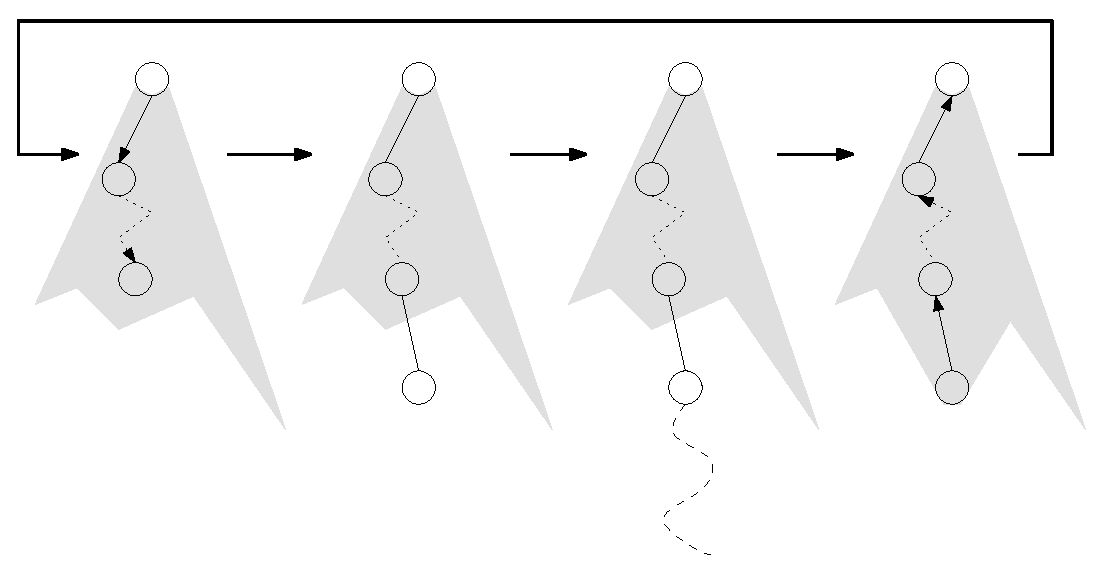
\includegraphics[width=0.7\textwidth]{figs/mcts.eps}\\
~ Selection ~~~~~~~ Expansion ~~~~~~~ Rollout ~~~~~~~ Update
\end{center}
{\small
\begin{itemize}
\item[Selection] A tree is asymmetrically grown toward the most promising region.\pause
\item[Expansion] Tree descended using an exploration/exploitation policy until a unexplored leaf found.\pause
\item[Rollout] Node added to the tree and solution completed by some procedure.\pause
\item[Update] Solution back-propagated to nodes on the path taken.
\end{itemize}}
\end{frame}

\section{Learning a Game Playing Policy using Data}



\begin{frame}{Decision Making in Board Games}
\begin{columns}[t]
\begin{column}{0.4\textwidth}
\begin{center}
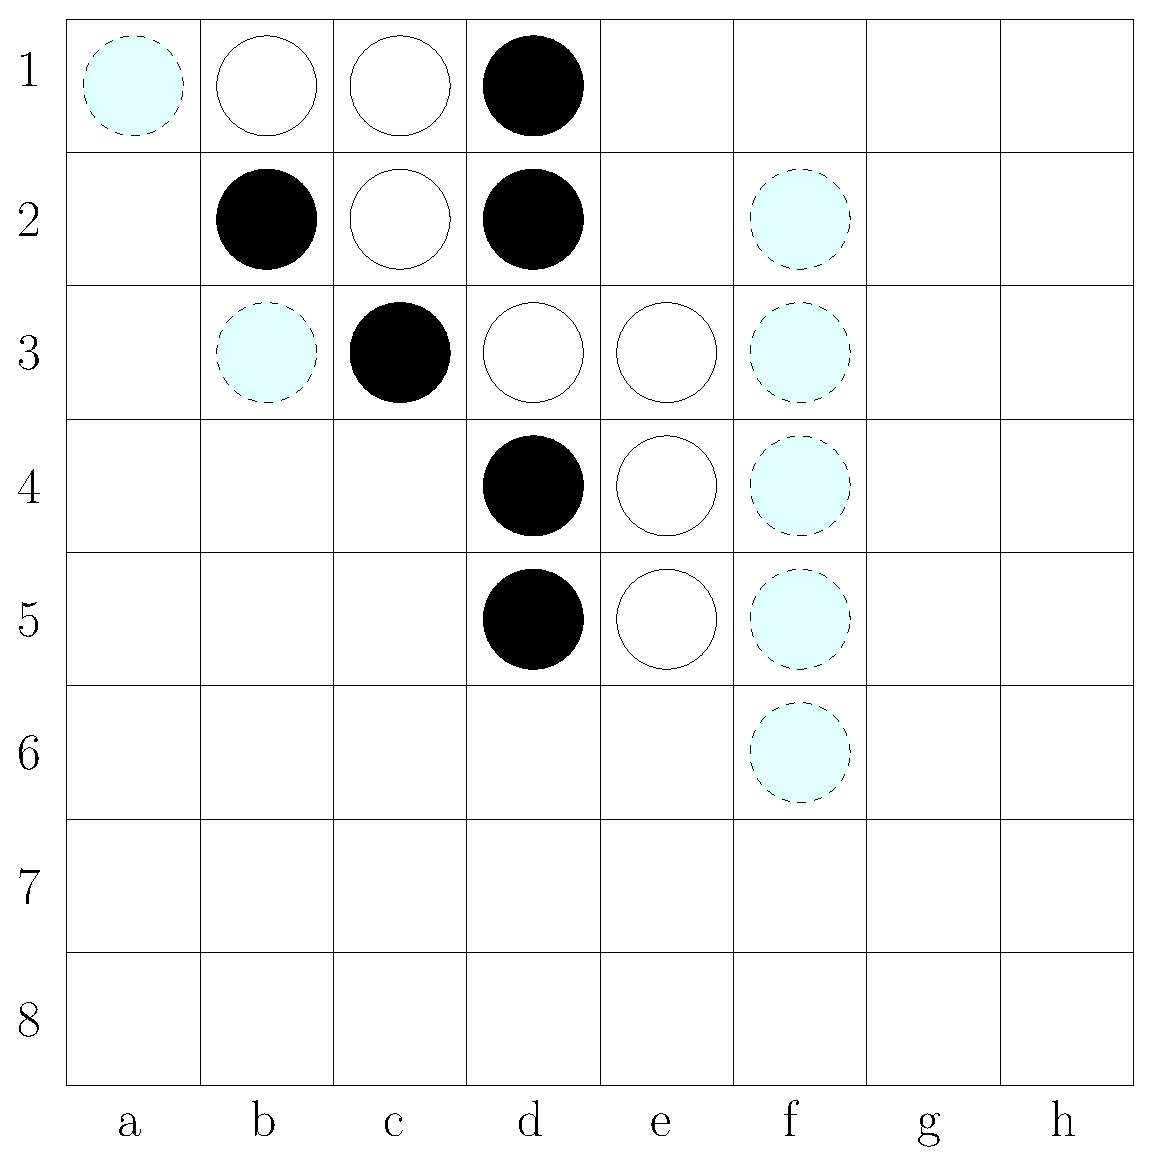
\includegraphics[width=\textwidth,]{figs/othello_ipe.eps}
\end{center}
\end{column}
\begin{column}{0.6\textwidth}
\ \\ \ \\ \ \\
Othello game in progress with seven possible legal moves for black (dash). 
\\ \ \\
The purpose of learning a board \underline{evaluation function} is to decide which move to take. \pause
\end{column}
\end{columns}

\ \\
\begin{itemize}
\item When used in a one-ply search or a minimax game tree, decisions are based on comparisons. \pause
\item The absolute values are not important, only relative values are needed.
%\item Insight: learning preferences may be easier to learn than attempting to learn absolute values.
\end{itemize}


\end{frame}


\begin{frame}{Preference Learning}

\begin{itemize}
\item Simply learn to satisfy constraints that lead to correct choices.\\ \ \pause
\item Don't care about absolute values.\\ \ \pause
\item What are correct choices?\\ \ \pause
\item Given a set of game logs (trajectories)\\ \
\item For each board state with more than one legal move:
\begin{itemize}
\item label board state reached by chosen move as \lq\lq correct\rq\rq.\pause
\item label all other board states reachable by a single legal move as \lq\lq incorrect\rq\rq.\pause
\end{itemize}
\item Attempt to learn a function that performs correct classification according to the above.
\end{itemize}


\end{frame}

\begin{frame}{A linear evaluation function based on $n$-tuples features}

\begin{center}
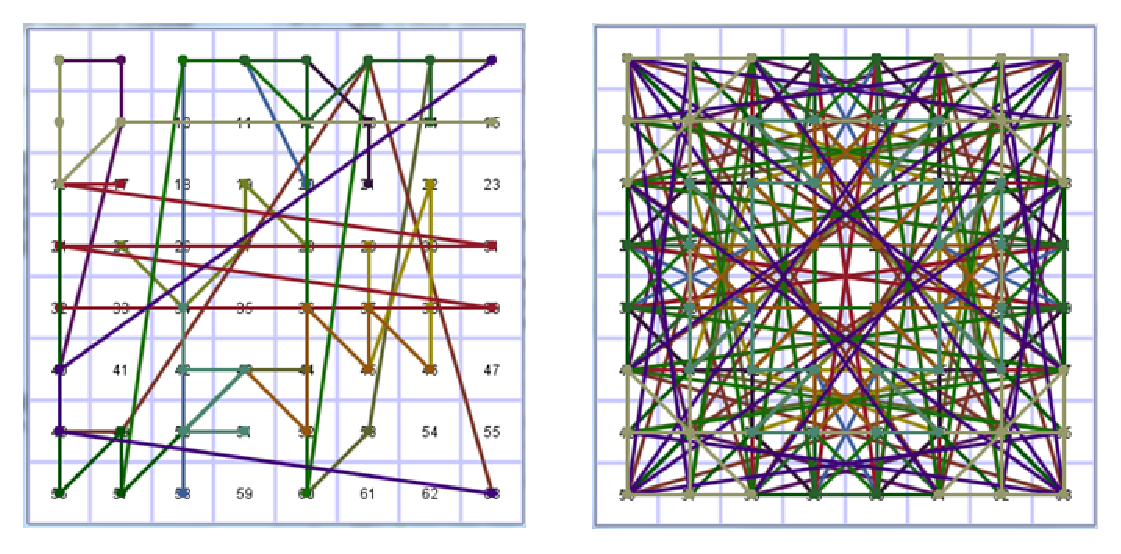
\includegraphics[width=0.8\textwidth,]{figs/NTupleSnakes.eps}
\end{center}

\begin{itemize}
\item Essentially a linear architecture with highly non-linear pattern-like features $\phi$. \pause
\item In our study we have used an $n$-tuple architecture evolved by Pete Burrow, with 6561 features.\pause
\item The evaluation function is simply $Q(s,a) = \vec{w}^\intercal \phi(s^a)$, where $s^a$ is the after or post-decision state when move $a$ is chosen.
\end{itemize}




\end{frame}



\begin{frame}{Preference Learning}

\noindent
Say that move $j$ is preferred to move $k$ then the learner simply aims to satisfy the simple constraint:

\begin{equation*}
  \vec{w}^\intercal \phi_j > \vec{w}^\intercal \phi_k
\end{equation*}

or solve the problem of minimizing $\| \vec{w} \|$ and satisfying
\begin{equation*}
  [\vec{w}^\intercal(\phi_j - \phi_k)] > 1 \; \forall j \in J, \; k \in K
\end{equation*}

where $J$ and $K$ are the preferred and non-preferred post-decision board states respectively.

\end{frame}


\begin{frame}{Other Machine Learning Approaches}

We (with Simon Lucas) have compared preference learning with the following approaches (and variations thereof):

\begin{itemize}
\item least squares temporal difference learning,\\ \
\item direct classification, \\ \
\item and the Bradley-Terry model fitted using minorization-maximization.
\end{itemize}


\end{frame}
 







%\section{Experiments}

\begin{frame}{Human Generated Expert Games Trajectories}

\begin{itemize}
\item Taken from human competitions held by the French Othello
Federation \href{http://www.ffothello.org/}{www.ffothello.org}.\\ \
\item More than 112 thousand games available, we use only one thousand. \\ \
\end{itemize}


\end{frame}


\begin{frame}{Matching human decisions (French Othello league)}

%\begin{table}[h!]
%\caption{The branching factor (BF) and number of training samples at different 
%game stages. The percentage of correct moves taken on testing data for the 
%hand crafted heuristic weights, ETDL-$n$tuple, the LSTD($\lambda$) and preference learning 
%weights, both using either WPC or $n$tuples.}\label{t:errors}
%\centering
{\footnotesize
\vspace{-.5cm}
\begin{tabular}{|c|rr|rrrr|rr|}
\hline
& & & $n$-Tuple & & &  & WPC & \\
\#discs & BF & \#N    & PREF & MM & LSTD  & Classify & & ETDL \\\hline
 1--16 & 7.1 & 73133   &  78.3  & 68.8 & 29.8 & 68.7 & 21.9 & 13.4\\ 
17--20 & 11.0 & 40045  & 52.4  & 43.0 & 15.2 & 31.8 & 2.6 & 15.5\\ 
21--24 & 11.5 & 42194  & 49.6  & 33.4 & 21.6 & 32.2 & 2.0 & 20.6\\ 
25--28 & 11.9 & 43796  & 45.1  & 31.1 & 20.7 & 34.1 & 5.2 & 22.9\\ 
29--32 & 11.7 & 42818  & 40.5  & 26.2 & 18.4 & 29.7 & 4.3 & 22.1\\ 
33--36 & 11.3 & 41319  & 40.1  & 28.0 & 17.6 & 30.2 & 6.8 & 24.9\\ 
37--40 & 10.6 & 38318  & 41.8  & 30.6 & 17.9 & 32.0 & 9.4 & 26.1\\ 
41--44 & 9.6 & 34308  & 41.5  & 31.6 & 20.4 & 32.5 & 14.3 & 29.6\\ 
45--48 & 8.4 & 29412  & 43.6  & 34.0 & 21.6 & 34.7 & 20.8 & 31.5\\ 
49--52 & 7.1 & 23784  & 44.0  & 35.3 & 24.1 & 36.4 & 27.2 & 35.8\\ 
53--56 & 5.5 & 17385  & 49.0  & 40.9 & 31.3 & 41.1 & 33.4 & 42.2\\ 
57--60 & 4.0 & 10960  & 53.9  & 46.5 & 39.0 & 48.3 & 38.7 & 49.5\\ 
61--64 & 2.5 & 3411   & 62.5  & 55.9 & 52.8  & 57.3 & 48.0 & 61.3\\ \hline
$\sum$ & 8.6 & (437883)  & 53.0  & 42.5 & 25.1 & 42.7 & 17.6 & 27.0  \\  
\hline 
\end{tabular}}


\end{frame}




%Cross Validation Accuracy = 83.4794% for othello league

%MCTS Cross Validation Accuracy = 68.0093%



\begin{frame}{Round Robin League}

\begin{itemize}
\item Each evaluation function was used to play each other one using one-ply minimax 
search from the same 1000 randomly chosen unique initial positions. \\ \ \pause
\item We then used BayesElo to rank the players and to assess the likelihood of superiority.\\ 
\end{itemize}


\end{frame}



\begin{frame}{Round Robin League Rating}

\begin{tabular}{|l|l|rr|c|r|}
\hline
Ranking & Player & Rating & \% Score   & b/w  & $|w|$   \\ \hline
1 & iPref-N-Tuple    & 1879 & 82.3\%   & inv  & 6,561   \\     
2 & ETDL-N-Tuple     & 1871	& 81.6\%   & neg  & 6,561   \\  
3 & Pref-N-Tuple     & 1779	& 72.3\%   & neg  & 6,561   \\
4 & Coev-WPC         & 1672	& 59.7\%   & neg  &    64   \\
5 & Heur-WPC         & 1655	& 57.5\%   & neg  &    64   \\
6 & MM-N-Tuple       & 1630	& 54.3\%   & inv  & 6,561   \\
7 & iPref-1-Tuple    & 1555 & 44.7\%   & inv  &   192   \\
8 & MM-1-Tuple       & 1542	& 43.0\%   & inv  &   192   \\
9 & Pref-1-Tuple     & 1511	& 39.1\%   & neg  &   192   \\
10 & Classify-N-Tuple & 1500 & 37.7\%  & inv  & 6,561 \\
11 & Classify-1-Tuple & 1425 & 28.5\%  & inv  &   192    \\ 
12 & LSTD-N-Tuple    & 1419	& 27.8\%   & neg  & 6,561   \\
13 & LSTD-1-Tuple    & 1360	& 21.6\%   & neg  &   192   \\ \hline
\end{tabular}


%Rank Name   Elo    +    - games score oppo. draws
%   1 PETE     151    6    6 14000   66%     0    0%
%   2 NTUPLE4     121    6    6 14000   63%     0    0%
%   3 BLEND      65    6    6 14000   57%     0    0%
%   4 PREF      14    6    6 14000   51%     0    0%
%   5 MCTS      12    6    6 14000   51%     0    0%
%   6 MCTS-T    -112    6    6 14000   38%     0    0%
%   7 HEUR    -251    7    7 14000   25%     0    0%
%
%P1 MCTS
%P2 HEUR
%P3 PREF
%P4 MCTS-TRAIN
%P5 BLEND
%P6 PETE
%P7 NTUPLE4




\end{frame}


\section{Data Driven Design of Composite Dispatching Rules}

\begin{frame}{Data Driven Design of Composite Dispatching Rules}

Use now the same preference learning technique for learning dispatching policies for scheduling problems:
\begin{itemize}
\item Generate optimal dispatching \lq\lq trajectories\rq\rq using a MIP solver (Gurobi). \\ \
\item Use random instance generator to create example problems to train on and others for testing. \\ \
\item We will look at 3 different types of scheduling problems.
\end{itemize}


\end{frame}

\begin{frame}{Jobshop processing times $U(1,100)$ order random}
  
\begin{center}
\includegraphics<1>[height=0.9\textheight]{../step_50_1.eps}%
\includegraphics<2>[height=0.9\textheight]{../step_50_2.eps}%
\includegraphics<3>[height=0.9\textheight]{../step_50_3.eps}%
\includegraphics<4>[height=0.9\textheight]{../step_50_4.eps}%
\includegraphics<5>[height=0.9\textheight]{../step_50_5.eps}%
\includegraphics<6>[height=0.9\textheight]{../step_50_6.eps}%
\includegraphics<7>[height=0.9\textheight]{../step_50_7.eps}%
\includegraphics<8>[height=0.9\textheight]{../step_50_8.eps}%
\includegraphics<9>[height=0.9\textheight]{../step_50_9.eps}%
\includegraphics<10>[height=0.9\textheight]{../step_50_10.eps}%

\end{center}

\end{frame}



\begin{frame}{Jobshop-$10\times 10$, $U(1,100)$ -- average decision accuracy}
\begin{center}
\includegraphics[width=0.8\textwidth,]{../jrnd.eps}
\end{center}

\end{frame}

\begin{frame}{Jobshop-$10\times 10$, $U(1,100)$ -- impact on objective}
\begin{center}
\includegraphics[width=0.8\textwidth,]{../jrnd_2.eps}
\end{center}

\end{frame}

\begin{frame}{Jobshop processing times $U(51,100)$ order random}
  
\begin{center}
\includegraphics<1>[height=0.9\textheight]{../narr_step_50_1.eps}%
\includegraphics<2>[height=0.9\textheight]{../narr_step_50_2.eps}%
\includegraphics<3>[height=0.9\textheight]{../narr_step_50_3.eps}%
\includegraphics<4>[height=0.9\textheight]{../narr_step_50_4.eps}%
\includegraphics<5>[height=0.9\textheight]{../narr_step_50_5.eps}%
\includegraphics<6>[height=0.9\textheight]{../narr_step_50_6.eps}%
\includegraphics<7>[height=0.9\textheight]{../narr_step_50_7.eps}%
\includegraphics<8>[height=0.9\textheight]{../narr_step_50_8.eps}%
\includegraphics<9>[height=0.9\textheight]{../narr_step_50_9.eps}%
\includegraphics<10>[height=0.9\textheight]{../narr_step_50_10.eps}%

\end{center}

\end{frame}

\begin{frame}{Jobshop-$10\times 10$, $U(51,100)$ -- average decision accuracy}
\begin{center}
\includegraphics[width=0.8\textwidth,]{../jrndn.eps}
\end{center}
\end{frame}

\begin{frame}{Jobshop-$10\times 10$, $U(51,100)$ -- impact on objective}
\begin{center}
\includegraphics[width=0.8\textwidth,]{../jrndn_2.eps}
\end{center}
\end{frame}


\begin{frame}{Permutation flow shop with processing times $U(1,100)$}
  
\begin{center}
\includegraphics<1>[height=0.9\textheight]{../flow_step_50_1.eps}%
\includegraphics<2>[height=0.9\textheight]{../flow_step_50_2.eps}%
\includegraphics<3>[height=0.9\textheight]{../flow_step_50_3.eps}%
\includegraphics<4>[height=0.9\textheight]{../flow_step_50_4.eps}%
\includegraphics<5>[height=0.9\textheight]{../flow_step_50_5.eps}%
\includegraphics<6>[height=0.9\textheight]{../flow_step_50_6.eps}%
\includegraphics<7>[height=0.9\textheight]{../flow_step_50_7.eps}%
\includegraphics<8>[height=0.9\textheight]{../flow_step_50_8.eps}%
\includegraphics<9>[height=0.9\textheight]{../flow_step_50_9.eps}%
%\includegraphics<10>[height=0.9\textheight]{../flow_step_50_10.eps}%

\end{center}

\end{frame}




\begin{frame}{Flowshop-$8\times 8$, $U(1,100)$ -- average decision accuracy}
\begin{center}
\includegraphics[width=0.8\textwidth,]{../frnd.eps}
\end{center}
\end{frame}





\begin{frame}{Flowshop-$8\times 8$, $U(1,100)$ -- impact on objective}
\begin{center}
\includegraphics[width=0.8\textwidth,]{../frnd_2.eps}
\end{center}

\end{frame}

\section{Discussion and Challenges}

\begin{frame}{Discussion and Challanges}

\begin{itemize}
\item Visualization techniques (analytics) for combinatorial optimization.\\ \ \pause
\item Problem specific feature discovery for combinatorial optimization.\\ \ \pause
\item Understanding where decision are critical for success (focus the training data).\\ \ \pause
\item Sub-optimal trajectory sampling? For games we have found that sampling more effectively the game state space is important.\\ \ \pause
\item Apply these techniques directly within MIP solvers such as Gurobi. We are currently investigating this using SCIP. \ \pause
\end{itemize}

\end{frame}


\end{document}
